\subsection{Resultados com Protótipo}

Como descrito na Seção \ref{subsec:prototipoExperimento} foram realizados dois testes com o protótipo, o primeiro utilizando uma infraestrutura fixa e outro só com os veículos.

A Figura demonstra a comparação entre as médias das latências, pode-se observar que a infraestrutura não causou nenhum impacto na latência. Isso ocorre pelo fato que ambos os experimentos utilizaram os mesmos algoritmos de locomoção do agente e equipamentos. Levando em consideração que o ambiente era controlado e não existiam outras fontes de ruído, o Zigbee apresentou uma baixa variação da latência. A Tabela \ref{tab:experimentoRealLatencia} apresenta informações como média e variância.


\begin{figure}[htbp]
	\centering
	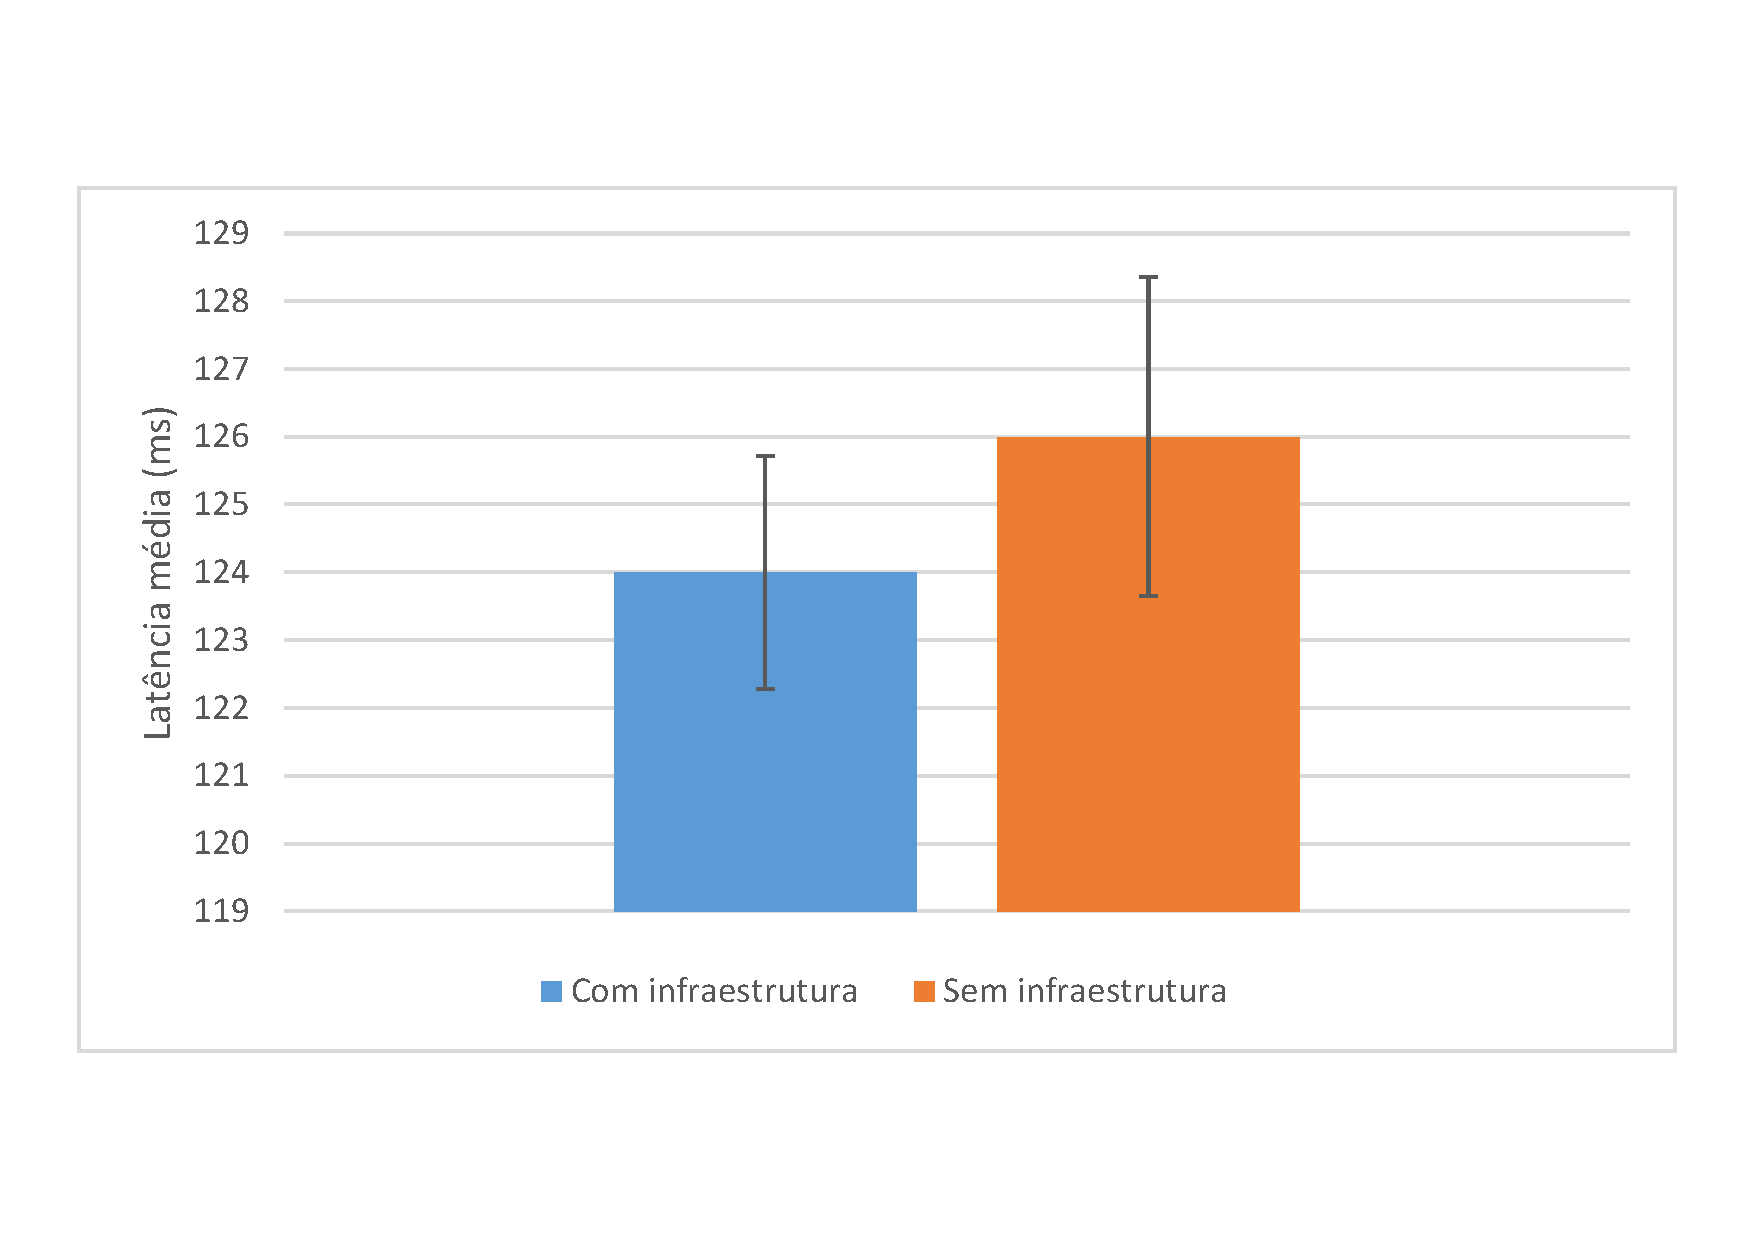
\includegraphics[scale=0.4]{resultados/graficos/experimentoRealLatencia.pdf}
	\caption{Latência obtida no experimento com o protótipo.}
	\label{fig:experimentoRealLatencia}
\end{figure}


\begin{table}[ht]
	\caption{Dados estatisticos da latência.}
	\centering
	\begin{tabular}{ | l | c | c | c|}
		\hline
		& média aritmetica & Desvio Padrão & Variância \\ \hline
		Sem infraestrutura & 126 (ms) & 2,3123 & 5,6288  \\ \hline
		Com infraestrutura & 124 (ms) & 1,7654 & 2,8354 \\ \hline
	\end{tabular}
	\label{tab:experimentoRealLatencia}
\end{table}

Com infraestrutura o agente realizou duzentos e setenta migrações e em vinte e nove o agente foi perdido. Quando é observado as migrações na situação sem infraestrutura o agente realizou duzentos e onze migrações e se perdeu em vinte e três migrações. A Tabela \ref{tab:migracoesPerda} demonstra o resultado da simulação em relação a migração e perda do agente.

\begin{table}[ht]
	\caption{Relação quantidade migração e perda.}
	\centering
	\begin{tabular}{ | l | c | c | c |}
		\hline
					& Migrações & Perda do agente & \% \\ \hline
		Sem infraestrutura & 211 & 45 & 21,32\%  \\ \hline
		Com infraestrutura & 270 & 23 & 10,74\%  \\ \hline
	\end{tabular}
	\label{tab:migracoesPerda}
\end{table}

O agente realiza mais migrações na situação com infraestrutura por que ela possui um nó a mais. Outro ponto importante é a porcentagem da taxa de perda do agente  em relação a quantidade de migração. Como a infraestrutura permanece estática, a velocidade relativa entre o nó no veículo e o nó da infraestrutura é a velocidade do veículo. Então o tempo que o agente tem para migrar e maior por que aumenta o tempo de comunicação entre os nós. No caso do experimento só com veículos a velocidade relativa é a soma das velocidades dos dois veículos, isso diminui o tempo que o agente tem para migrar, causando o aumento da perda do agente. As Figuras \ref{fig:velocidadeRelativaNegativa}, \ref{fig:velocidadeRelativaPositiva} e \ref{fig:velocidadeRelativaNeutra} exemplificam a velocidade relativa.


\begin{figure}[htbp]
	\centering
	\begin{minipage}{0.46\textwidth}
		\centering
		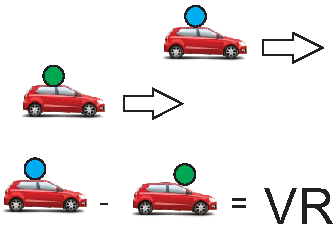
\includegraphics[scale=0.5]{resultados/figuras/velocidadeRelativaNegativa.pdf}
		\captionof{figure}{VR negativa.}
		\label{fig:velocidadeRelativaNegativa}
	\end{minipage}
	\begin{minipage}{0.46\textwidth}
		\centering
		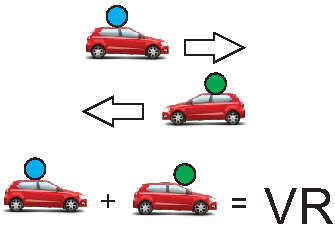
\includegraphics[scale=0.5]{resultados/figuras/velocidadeRelativaPositiva.pdf}
		\captionof{figure}{VR positiva.}
		\label{fig:velocidadeRelativaPositiva}
	\end{minipage}
	\begin{minipage}{0.46\textwidth}
		\centering
		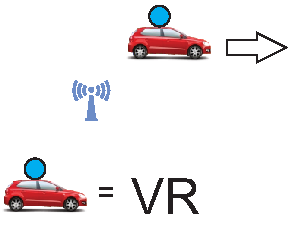
\includegraphics[scale=0.5]{resultados/figuras/velocidadeRelativaNeutra.pdf}
		\captionof{figure}{VR neutra.}
		\label{fig:velocidadeRelativaNeutra}
	\end{minipage}
\end{figure} 